\documentclass[main.tex]{subfiles}
\begin{document}

\chapter{Results}
The results of the numerical experiments will be presented in this chapter.
For both optimization targets the optimized pulses, their properties and the final evolved state will be presented.


\section{Qubit state transfers}
\subsection{\texorpdfstring{\boldmath\( \ket{1}_q\ket{0}_r\rightarrow\ket{0}_q\ket{C_1}_r \)}{10 -> 0C1} state transfer}
In \cref{fig:3d-optim-ge} the fidelity during all optimization runs are plotted.
For pulse lengths longer than \SI{15}{\nano\second} the fidelity starts at values close to the goal (\(F>0.9\)) and the number of iterations is relatively low (less than 85 iterations).
In contrast, pulses shorter than \SI{15}{\nano\second} start at lower fidelities while the number of iterations are roughly one order of magnitude larger with no clear pattern.

To give a more detailed picture, the starting fidelity and optimized fidelity is plotted over pulse length in \cref{fig:fidelity-length-ge}.
The optimizations where the fidelity goal was not reached, pulse lengths equal to and below \SI{10.50}{\nano\second}, are marked with stars.
%The drop-off in fidelity for shorter pulses is linear.

\begin{figure}
    \centering
    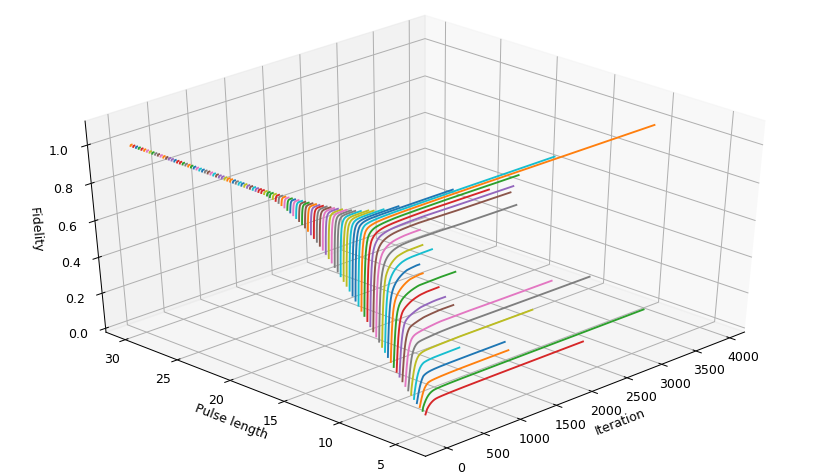
\includegraphics[width=\linewidth]{figs/3d-optim-ge.png}
    \caption{Fidelity during optimizations for every pulse length (ns). The different colors help distinguish the lines.}\label{fig:3d-optim-ge}
\end{figure}

\tikzfig{figs/fidelity-length-ge}{%
Fidelity of first and last iteration of every pulse length.
The stable region above 
}{fig:fidelity-length-ge}{\textwidth}{15em}

Further analysis is done on pulses with lengths \SI{4.25}{\nano\second}, \SI{6.0}{\nano\second}, \SI{8.0}{\nano\second}, \SI{10.0}{\nano\second}, \SI{20.0}{\nano\second} and \SI{30.0}{\nano\second}.
The optimized pulse shapes \(\text{Re}(\Omega)\) and \(\text{Im}(\Omega)\) are plotted in \cref{fig:pulse_shape} together with the guess pulses. Pulses longer than \ns{20} require only fine adjustments to the Blackman guess pulse while shorter pulses have an imaginary part which is maximized for the whole duration of the pulse.

\begin{figure}[ht]
\centering
\foreach \n/\capn [count=\ni] in {{4,25}/{4.25},{6,0}/{6.0},{8,0}/{8.0},{10,0}/{10.0},{20,0}/{20.0},{30,0}/{30.0}}{
	\subcaptionbox{Pulse length \capn{} ns}{
		\centering
		\setlength\figureheight{9.75em}
		\setlength\figurewidth{0.45\textwidth}
		\input{figs/pulse_shape_\n_Real.tikz}
		\input{figs/pulse_shape_\n_Imag.tikz}
	}%
	\ifnum\ni=6%
	        %
	\else%
		\hfill
	\fi%
}
\caption{Optimised pulse shapes and guess pulses for pulse lengths 
\textbf{(a)} \SI{4.25}{\nano\second}, 
\textbf{(b)} \SI{6.0}{\nano\second}, 
\textbf{(c)} \SI{8.0}{\nano\second}, 
\textbf{(d)} \SI{10.0}{\nano\second}, 
\textbf{(e)} \SI{20.0}{\nano\second}, 
and \textbf{(f)} \SI{30.0}{\nano\second}.
Short pulses (\(<\)\ns{10}) change substantially from the starting Blackman shape while long pulses (\(>\)\ns{20}) only require fine adjustments.}%
\label{fig:pulse_shape}
\end{figure}

The spectrum of \(\Omega(t)\) in the lab frame (\(\Omega(t)\ex^{i\omega_q t}\)) is shown in \cref{fig:pulse_spectrum}.
For all pulse lengths there is a peak centered roughly at \(\omega_q\) and the width of the peak becomes narrower for longer pulses.
For the highest pulse length \ns{30} there is almost no support at \(\omega_{02}\) and \(\omega_{12}\).

\begin{figure}[H]
\centering
\foreach \n/\capn [count=\ni] in {{4,25}/{4.25},{6,0}/{6.0},{8,0}/{8.0},{10,0}/{10.0},{20,0}/{20.0},{30,0}/{30.0}}{
	\subcaptionbox{Pulse length \capn{} ns}{
		\centering
		\setlength\figureheight{10em}
		\setlength\figurewidth{0.47\textwidth}
		\input{figs/pulse_spectrum_\n.tikz}
	}%
	\ifnum\ni=6%
	        %
	\else%
		\hfill
	\fi%
}
\caption{Pulse spectrum of the complex pulses in \cref{fig:pulse_shape}. The vertical lines indicate (from left to right) \(\omega_{02}\), \(\omega_{12}\), \(\omega_q\).}\label{fig:pulse_spectrum}
\end{figure}

The time evolution of the system under the optimized pulses are visualized by plotting the occupation of the states over time, \cref{fig:qubit_occupation},
the projection of the state on the Bloch sphere over time, \cref{fig:bloch_evolution}, and
a Hinton diagram of the evolved final state, \cref{fig:hinton}.

\begin{figure}[H]
\centering
\foreach \n/\capn [count=\ni] in {{4,25}/{4.25},{6,0}/{6.0},{8,0}/{8.0},{10,0}/{10.0},{20,0}/{20.0},{30,0}/{30.0}}{
	\subcaptionbox{Pulse length \capn{} ns}{
		\centering
		\setlength\figureheight{15em}
		\setlength\figurewidth{0.47\textwidth}
		\input{figs/qubit_occ_\n.tikz}
	}%
	\ifnum\ni=6%
	        %
	\else%
		\hfill
	\fi%
}
\caption{Energy level occupation over time for different lengths of optimized pulses.}\label{fig:qubit_occupation}
\end{figure}

For short pulse lengths there is not enough time for the transfer from \(\ket{0}\) to \(\ket{1}\),
but for a pulse length of roughly \ns{10.0} the goal is reached.
\Cref{fig:qubit_occupation} \textbf{(b)} shows a little rise in occupation of \(\ket{2}\) around \ns{7.5}. 

\begin{figure}[H]
\centering
\foreach \n/\capn [count=\ni] in {{4,25}/{4.25},{6,0}/{6.0},{8,0}/{8.0},{10,0}/{10.0},{20,0}/{20.0},{30,0}/{30.0}}{
	\subcaptionbox{Pulse length \capn{} ns}{\includegraphics[width=0.3\linewidth]{figs/bloch_evolution_\n.png}}%
	\ifnum\ni=6%
	        %
	\else%
		\hfill
	\fi%
}
\caption{Time dynamics on the Bloch sphere for different lengths of optimized pulses.}\label{fig:bloch_evolution}
\end{figure}

Looking at \cref{fig:bloch_evolution} we see that the transfer occurs along the y-axis for longer pulses.

\begin{figure}[H]
	\centering
	\foreach \n/\capn [count=\ni] in {{4,25}/{4.25},{6,0}/{6.0},{8,0}/{8.0},{10,0}/{10.0},{20,0}/{20.0},{30,0}/{30.0}}{
		\subcaptionbox{Pulse length \capn{} ns}{
			\centering
			\setlength\figureheight{0.30\textwidth}
			\setlength\figurewidth{0.30\textwidth}
			\input{figs/hinton_\n.tikz}
		}%
		\ifnum\ni=6%
				%
		\else%
			\hfill
		\fi%
	}
	\caption{Hinton diagram of \(\op{\psi(T)}\)}\label{fig:hinton}
\end{figure}

The Hinton diagram in \cref{fig:hinton} provides a visualization of the density matrix \( \op{\psi(T)} \).
The final density matrix shows how the much of the state is in the 

\clearpage{}
\section{%
	\texorpdfstring{\boldmath{\(\ket{0}\rightarrow\ket{2}\)}}{0 -> 2} state transfer
}

\begin{figure}
    \centering
    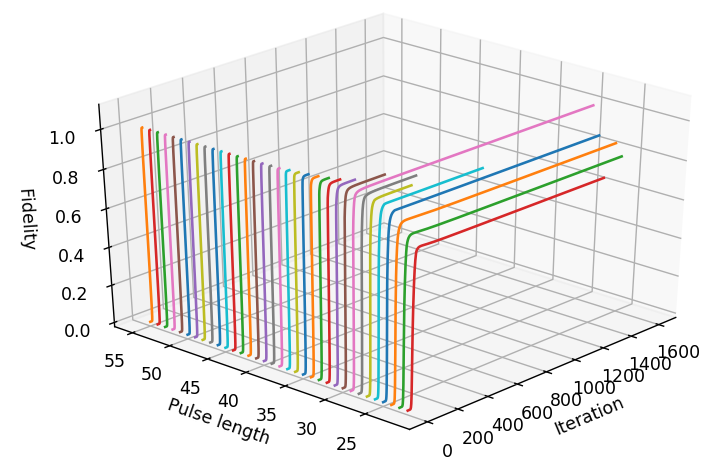
\includegraphics[width=0.7\linewidth]{figs/3d-optim-gf.png}
    \caption{Fidelity during optimizations for every pulse length (ns).}\label{fig:3d-optim-gf}
\end{figure}

\tikzfig{figs/fidelity-length-gf}{
Fidelity of first and last iteration of every pulse length.
}{fig:fidelity-length-gf}{0.8\textwidth}{15em}

\begin{figure}[ht]
\centering
\foreach \n/\capn [count=\ni] in {{22,0}/{22.0},{24,0}/{24.0},{26,0}/{26.0},{28,0}/{28.0},{29,0}/{29.0},{55,0}/{55.0}}{
	\subcaptionbox{Pulse length \capn{} ns}{
		\centering
		\setlength\figureheight{10em}
		\setlength\figurewidth{0.45\textwidth}
		\input{figs/pulse_shape_gf_\n_Real.tikz}
		\input{figs/pulse_shape_gf_\n_Imag.tikz}
	}%
	\ifnum\ni=6%
	        %
	\else%
		\hfill
	\fi%
}
\caption{Pulse shapes.}\label{fig:pulse_shape_gf}
\end{figure}


\begin{figure}[ht]
\centering
\foreach \n/\capn [count=\ni] in {{22,0}/{22.0},{24,0}/{24.0},{26,0}/{26.0},{28,0}/{28.0},{29,0}/{29.0},{55,0}/{55.0}}{
	\subcaptionbox{Pulse length \capn{} ns}{
		\centering
		\setlength\figureheight{10em}
		\setlength\figurewidth{0.47\textwidth}
		\input{figs/pulse_spectrum_gf_\n.tikz}
	}%
	\ifnum\ni=6%
	        %
	\else%
		\hfill
	\fi%
}
\caption{Pulse spectrum}%
\label{fig:pulse_spectrum_gf}
\end{figure}


\begin{figure}[ht]
\centering
\foreach \n/\capn [count=\ni] in {{22,0}/{22.0},{24,0}/{24.0},{26,0}/{26.0},{28,0}/{28.0},{29,0}/{29.0},{55,0}/{55.0}}{
	\subcaptionbox{Pulse length \capn{} ns}{
		\centering
		\setlength\figureheight{15em}
		\setlength\figurewidth{0.45\textwidth}
		\input{figs/qubit_occ_gf_\n.tikz}
	}%
	\ifnum\ni=6%
	        %
	\else%
		\hfill
	\fi%
}
\caption{Energy level occupation over time for different lengths of optimized pulses.}%
\label{fig:qubit_occupation_gf}
\end{figure}

\begin{figure}[ht]
\centering
\foreach \n/\capn [count=\ni] in {{22,0}/{22.0},{24,0}/{24.0},{26,0}/{26.0},{28,0}/{28.0},{29,0}/{29.0},{55,0}/{55.0}}{
	\subcaptionbox{Pulse length \capn{} ns}{
		\centering
		\setlength\figureheight{0.30\textwidth}
		\setlength\figurewidth{0.30\textwidth}
		\input{figs/hinton_gf_\n.tikz}
	}%
	\ifnum\ni=6%
	        %
	\else%
		\hfill
	\fi%
}
\caption{Hinton diagram of \(\op{\psi(T)}\)}%
\label{fig:hinton_gf}
\end{figure}

\clearpage{}
\subsection{\texorpdfstring{\boldmath\( \ket{1}_q\ket{0}_r\rightarrow\ket{0}_q\ket{C_1}_r \)}{10 -> 0C1} state transfer}
In this composite system it can be hard to see


\tikzfig{figs/cat_qubit_occ_80,0}{Occupation probability of the qubit over time.}{fig:cat_qubit_occ}{\textwidth}{15em}

\tikzfig{figs/cat_res_occ_80,0}{Occupation probability of the resonator over time.}{fig:cat_res_occ}{\textwidth}{15em}


Larger Hilbert space with the L=3 solution gives fidelities


\end{document}
